
\begin{frame}
    \frametitle{Maneuver execution}
    The maneuver is executed via a \structure{bi-level} control strategy\footcite{Duret2018a:JMT}:
    \begin{description}
      \item[Tactical layer]  Takes decision at the traffic level.  
      \item[Operational layer] Operates vehicles and control its acceleration. 
    \end{description}
    \vspace{-1cm}
    \begin{columns}
      \begin{column}{0.5\textwidth}
          \only<1|handout:0>{
          \begin{figure}
              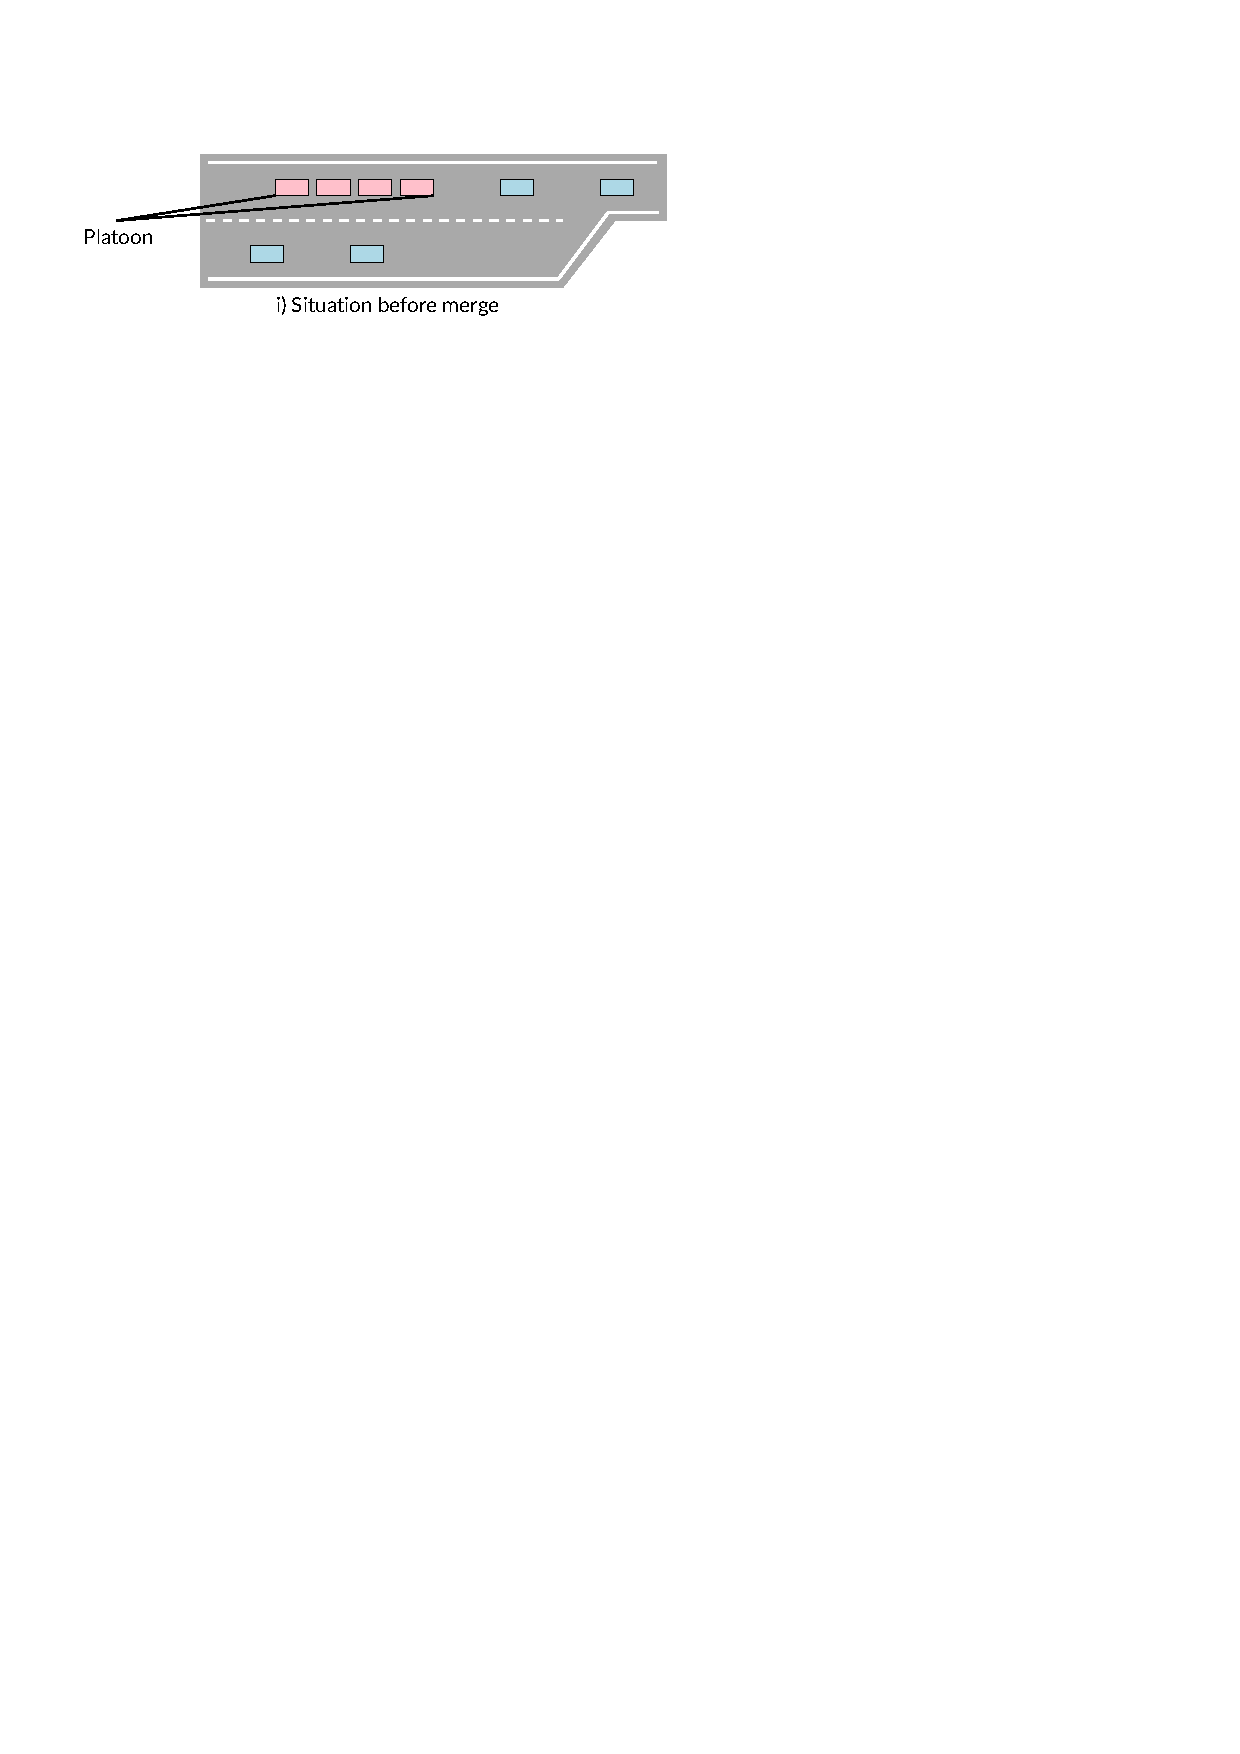
\includegraphics[width=\linewidth]{fig_5a_merge-phases.pdf}\hspace*{2cm} 
          \end{figure}
          }
          \only<2|handout:0>{
          \begin{figure}
            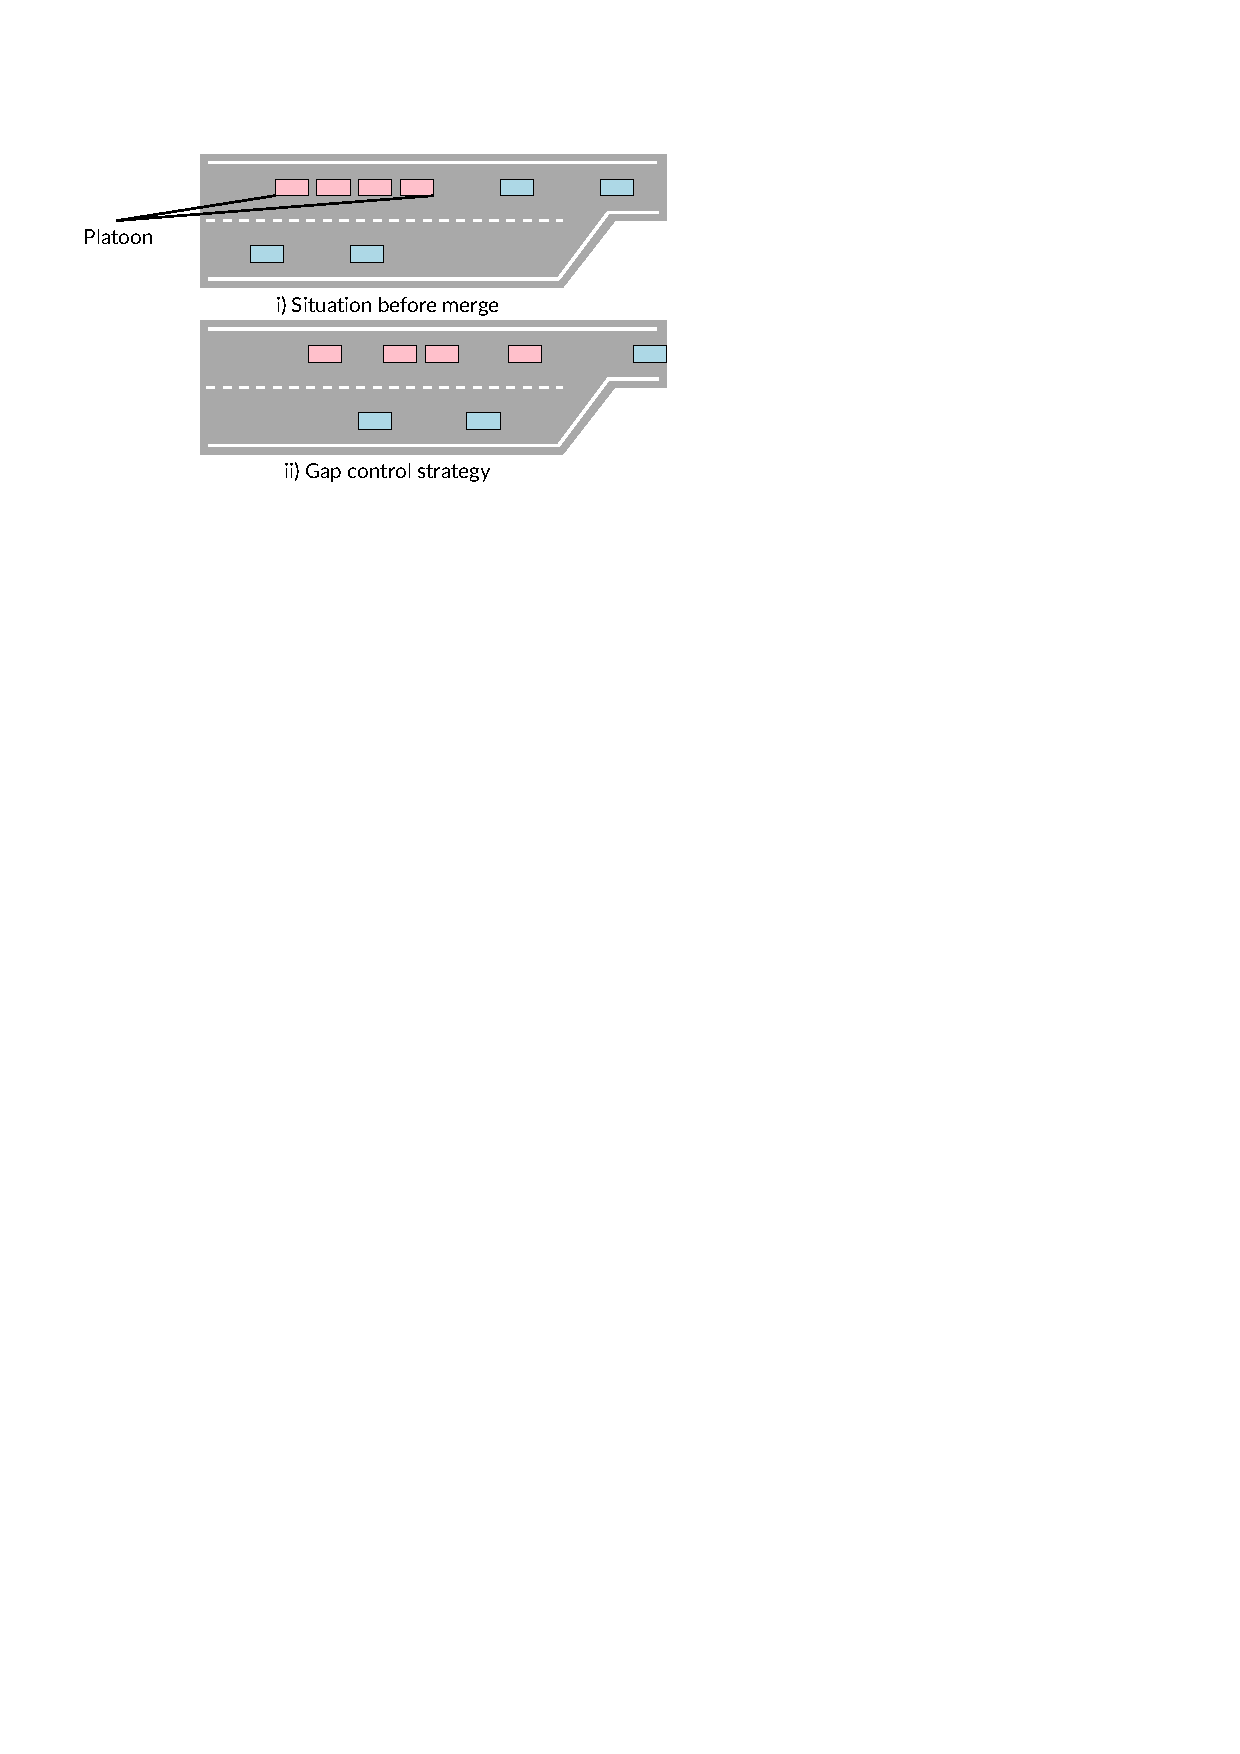
\includegraphics[width=\linewidth]{fig_5b_merge-phases.pdf}\hspace*{2cm} 
          \end{figure}
          }
          \only<3|handout:1>{
          \begin{figure}
            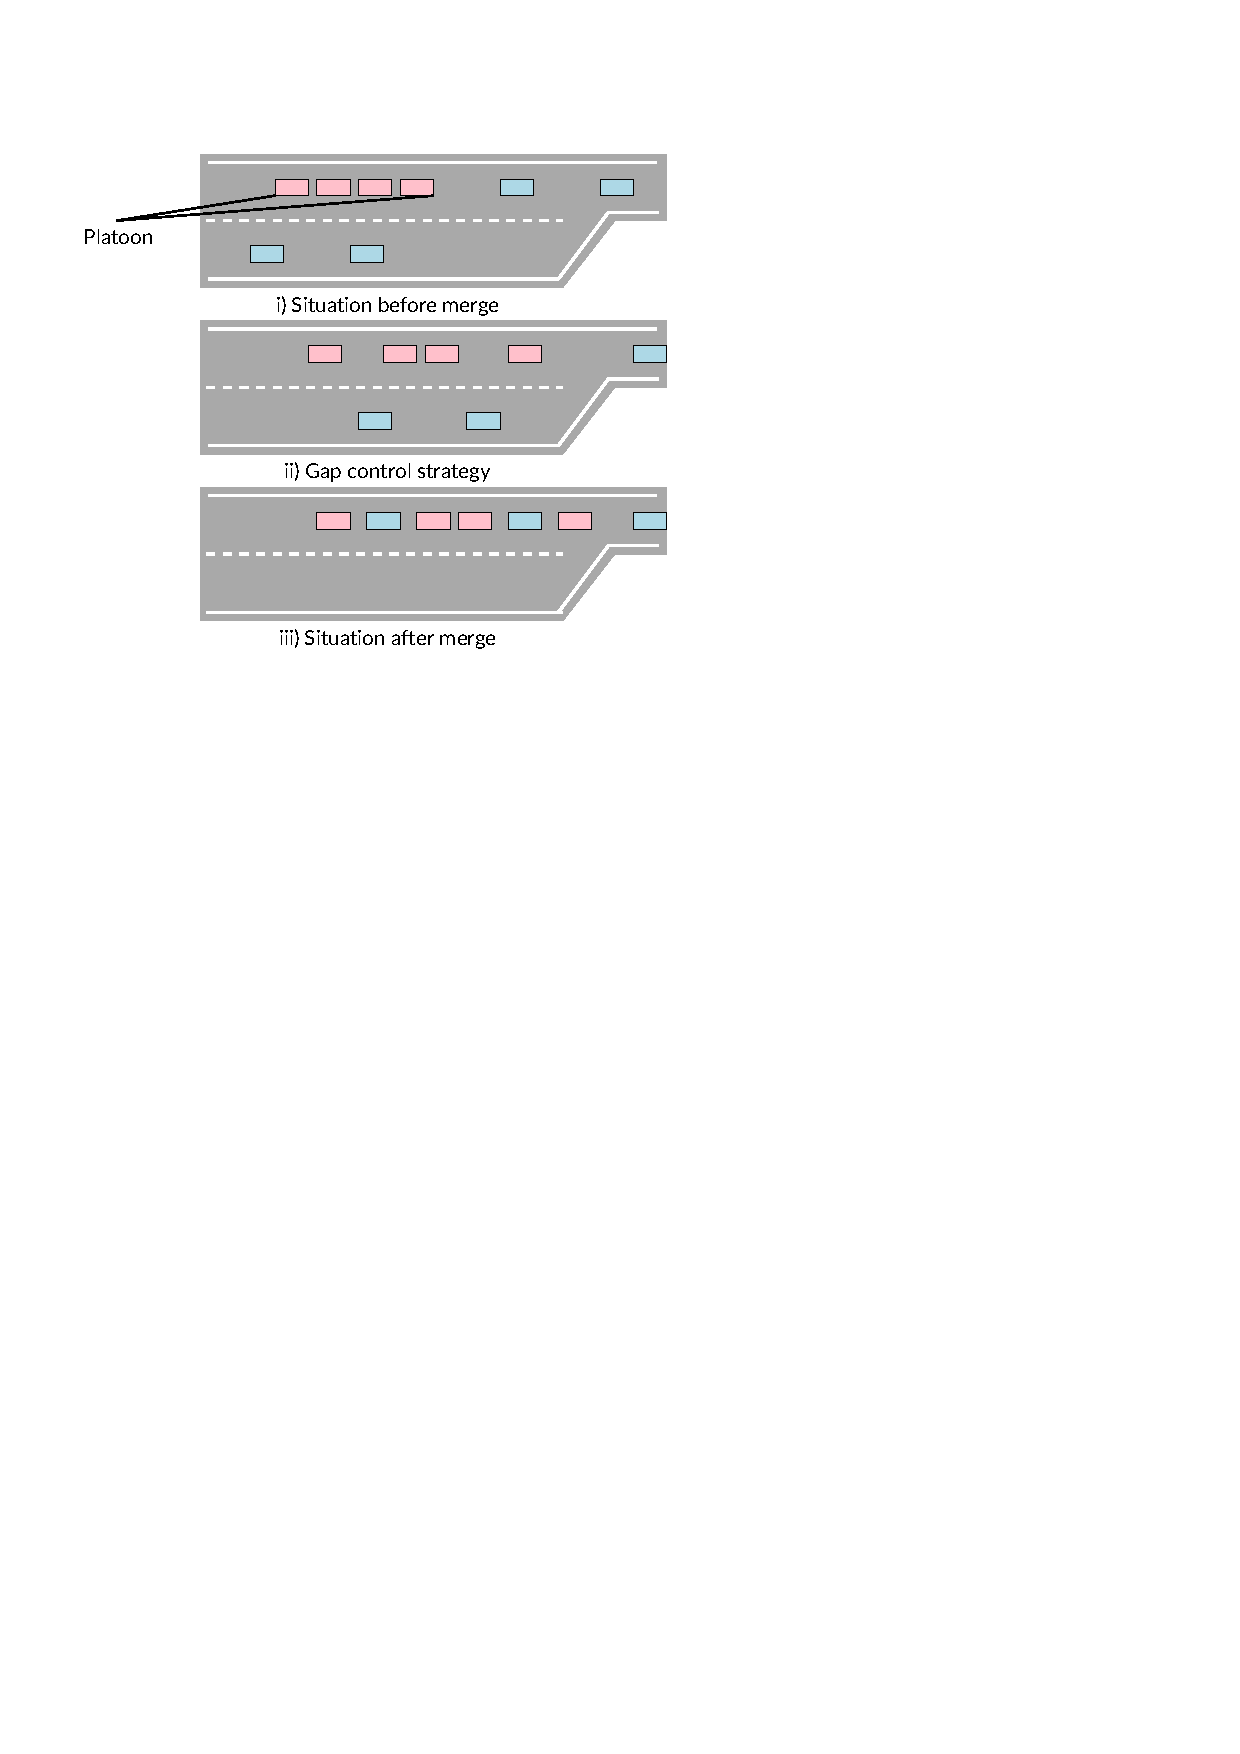
\includegraphics[width=\linewidth]{fig_5c_merge-phases.pdf}\hspace*{2cm} 
          \end{figure}
          }
      \end{column}
      \begin{column}{0.5\textwidth}
        \begin{figure}
          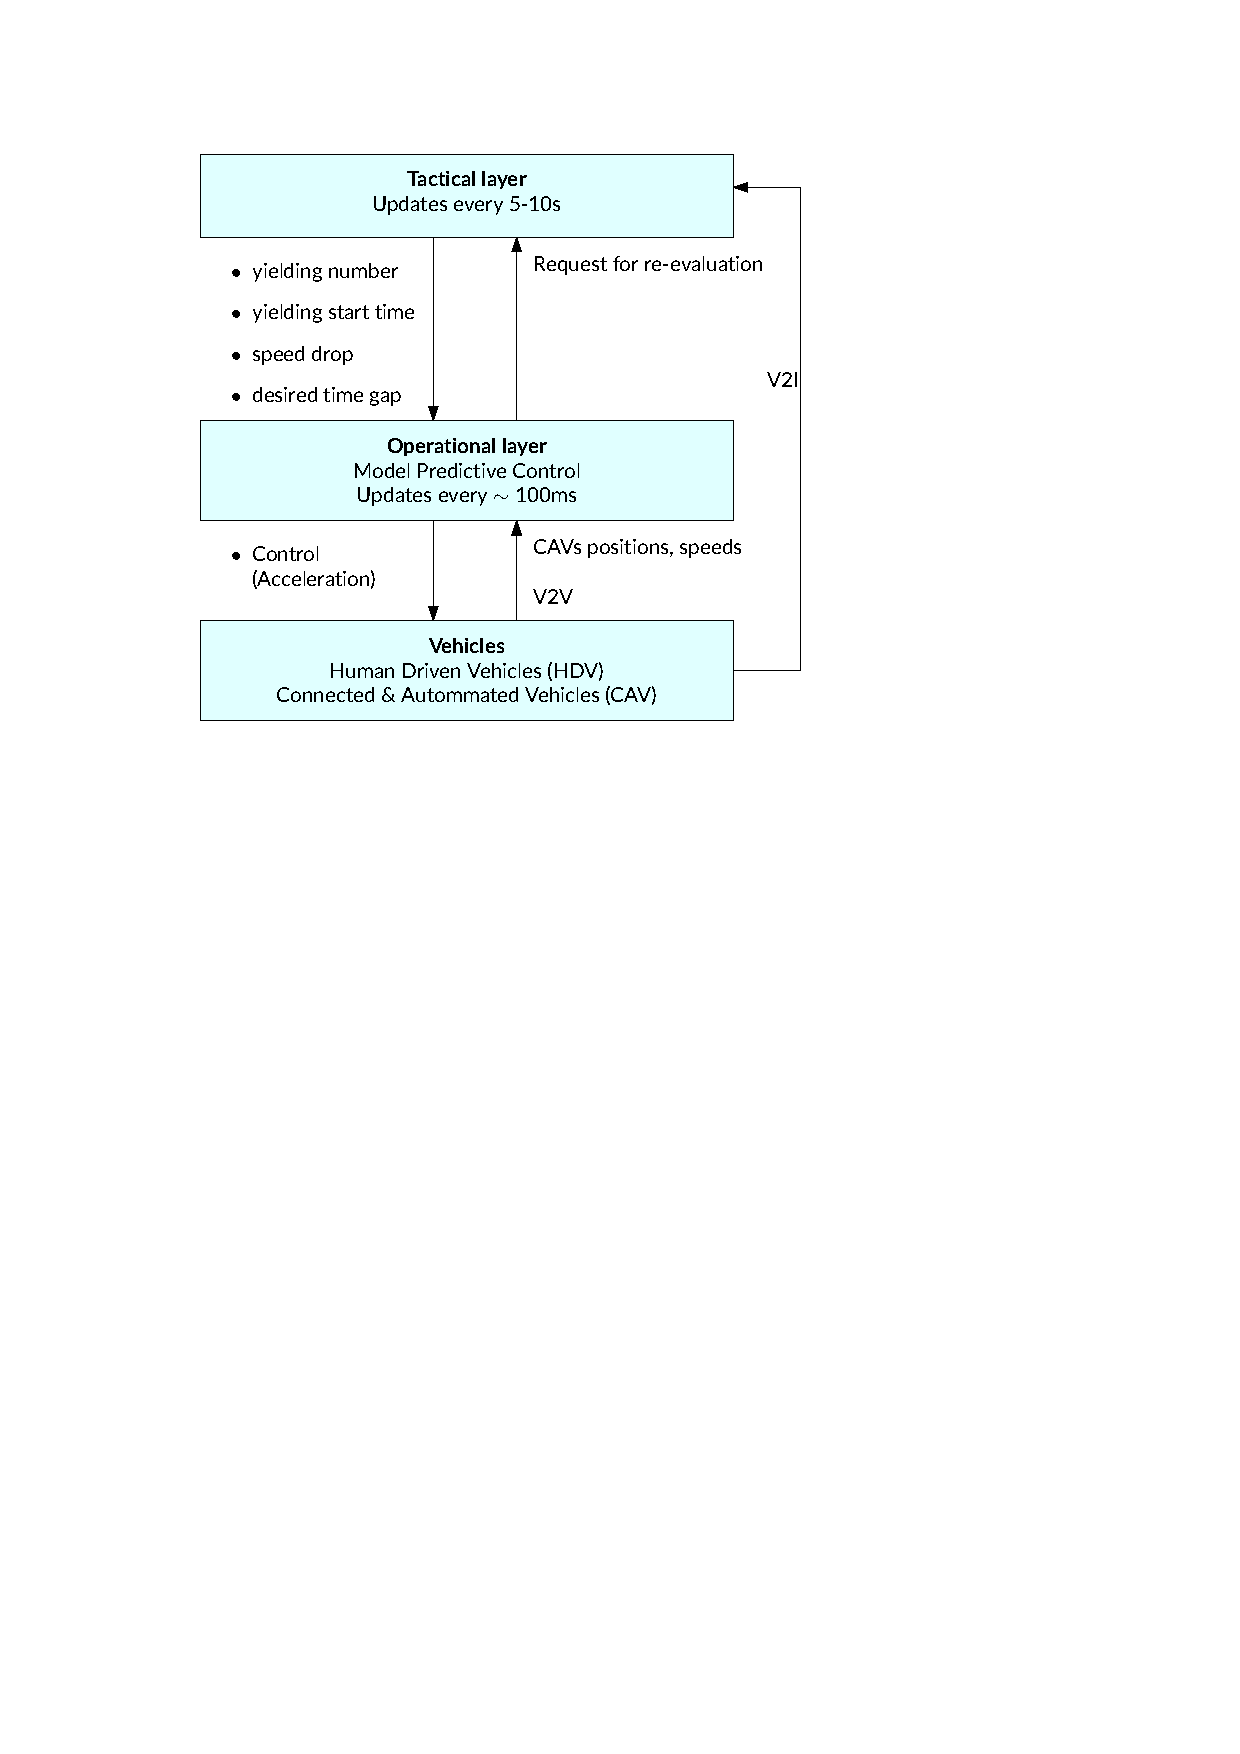
\includegraphics[width=0.9\linewidth]{fig_6_bilevel-strategy.pdf}\hspace*{2cm} 
        \end{figure}
      \end{column}
    \end{columns}
\end{frame}